\documentclass[tikz,border=2mm]{standalone}
\begin{document}
	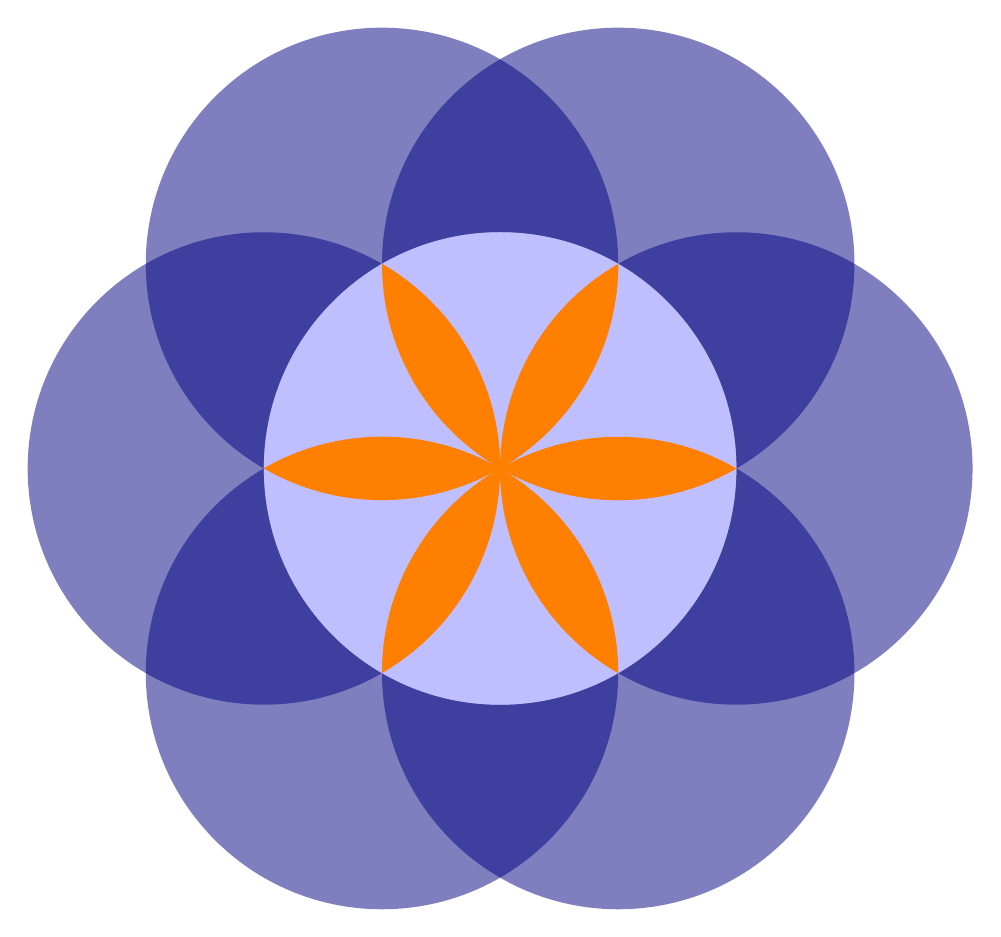
\begin{tikzpicture}
		[line join=round, line cap=round,line width=1pt]
		\def\r{3}
		\foreach \k in {1,2,3,4,5,6}
		\fill[blue!50!black, opacity=0.5] (\k*60:\r) circle (\r);
		\fill[white] (0,0) circle (\r);
		\fill[blue!50, opacity=0.5] (0,0) circle (\r);
		\foreach \k in {1,2,3,4,5,6}
		\fill[orange] (0,0) arc ((\k-1)*60:\k*60:\r)
		arc ((\k+2)*60:(\k+4)*60:\r);
	\end{tikzpicture}
\end{document}